\chapter{Extraktion raumakustischer Parameter}
\section{Die Nachhallzeit $\mathbf{RT_{60}}$}
\label{sec:rt60}Wir analysieren die Impulsantwort des Raumes HFT616 der TU Berlin.
Das Signal hat eine Abtastrate von $f_s$ = 44100 Hz und enthält am Anfang einen Bereich mit Grundrauschen bevor die eigentliche Impulsantwort beginnt.
Als erstes entfernen wir diesen Teil des Signals.
Als Kriterium zur Bestimmung des zeitlichen Nullpunkts der Impulsantwort verwenden die Position des ersten lokalen Maximums vor dem absoluten Maximum .
Zur Bestimmung der Nachhallzeit der gegebenen Impulsantwort haben wir die Schroeder Methode \cite{Schroeder65} verwendet.
Dazu haben wir in Matlab folgende Gleichung implementiert:

\begin{align*}
R[n] = \sum_{i=1}^N h^2[i] + \sum_{i=1}^n h^2[i]
\end{align*}
Aus diesem Vektor lässt sich wiederum eine diskretisierte Form der Energy Decay Curve berechnen, welche den auf 0 dB normierten Pegelabfall des Signals  beschreibt:
\begin{align*}
EDC_{norm}[n] = 10 \cdot \mathrm{log}_{10} \left(\frac{R[n]}{\sum_{i=1}^N h^2[i]}\right)
\end{align*}
Um daraus nun einen Wert für die Nachhallzeit T$_{60}$ zu bestimmen, haben wir T$_{20}$ und T$_{30}$ berechnet.
Dabei haben wir zunächst Indexdifferenzen gebildet und diese dann in Zeitwerte umgerechnet.
Für T$_{20}$ haben wir die Punkte die Pegelabfällen zwischen -5 dB und -25 dB in $EDC_{norm}[n]$ entsprechen verwendet, für T$_{30}$, die Differenz zwischen den -5 dB und -35 dB Punkten.
Dieses Vorgehen entspricht der DIN Norm 18041 \cite{DIN_18041}.
Die Ergebnisse für die Nachhallzeit sind in Tabelle \ref{tab:T} dargestellt.

\begin{table}[H]
\centering
\caption{Nachhallzeit}
\label{tab:T}
\begin{tabular}{ | c | c |}
  \hline
  T$_{60}$ aus T$_{20}$ &  0,79 s \\
  T$_{60}$ aus T$_{30}$ &  0,86 s \\
  \hline
  \end{tabular}
\end{table}


\begin{figure}[H]
    \center
    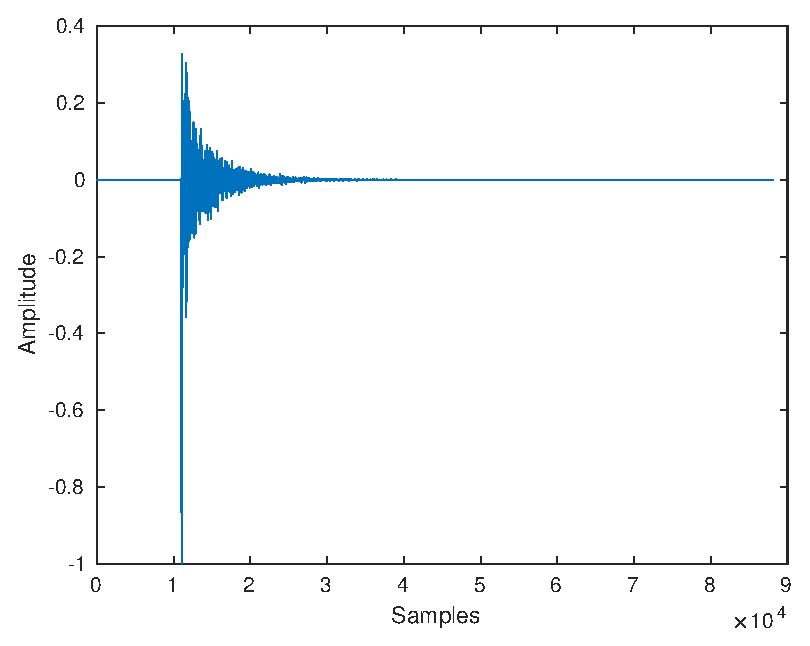
\includegraphics[width = 0.7\textwidth]{figures/samples}
    \caption{Die Impulsantwort}
    \label{fig:im}
\end{figure}

\begin{figure}[H]
    \center
    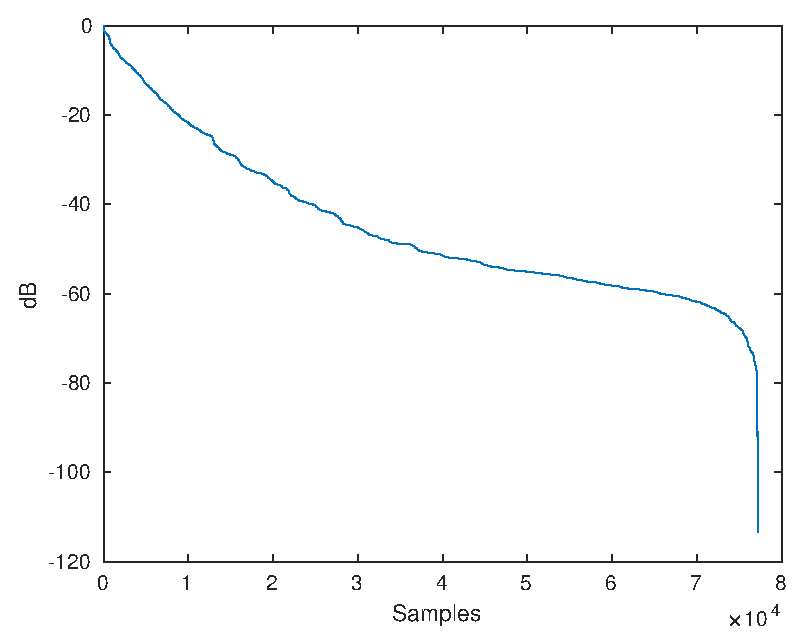
\includegraphics[width = 0.7\textwidth]{figures/EDC_norm.eps}
    \caption{EDC norm}
    \label{fig:edc}
\end{figure}

\section{Das Bassverhältnis $\mathbf{BR}$}
\label{sec:br}
Um das Bassverhältnis zu bestimmen ermitteln wir die Nachhallzeiten in verschiedenen Frequenzbereichen. Dazu filtern wir die Impulsantwort in Oktavbändern.
Wir generieren also vier neue Signale mittels Butterworth-Filtern dritter Ordnung mit Mittenfrequenzen bei 125 Hz, 250 Hz, 500 Hz und 1000 Hz. Auf diese wenden wir dieselbe Routine, wie in Aufgabe A) an, beschränken uns aber auf die Berechnung mittels $T_{20}$, um daraus die Nachhallzeiten $T_{60}$ zu erhalten:
\begin{table}[H]
\centering
\caption{Nachhallzeiten für Oktavbänder}
\label{tab:T_band}
\begin{tabular}{ | c | c |}
\hline
  Frequenzband & $T_{60}$ \\
  \hline
  125 Hz &  0,94 s \\
  250 Hz & 0,63 s \\
  500 Hz & 0,67 s \\
  1000 Hz & 0,61 s  \\
  \hline
  \end{tabular}
\end{table}

Für das Bassverhältnis BR folgt somit:
\begin{align*}
BR = \frac{T_{125 \mathrm{Hz}} + T_{250 \mathrm{Hz}}}{T_{500 \mathrm{Hz}} + T_{1000 \mathrm{Hz}}} = 1,23
\end{align*}  
Laut dem Handbuch der Audiotechnik \cite{Weinzierl08} (S. 191) wird solch ein Wert bei Musikaufführungsräumen angestrebt, in welchen der $BR$-Wert zwischen 1.0 und 1.3 liegen sollte.
Für Sprache hingegen sollte der Wert unterhalb von 1.0 liegen.

\section{Das Klarheitsmaß $\mathbf{C_{80}}$}
\label{sec:c80}
Für dieselben oktavbandgefilterten Signale, wie in Aufgabenteil B) können wir nun das Klarheitsmaß $C_{80}$ für die vier Frequenzbänder bestimmen.
Dieses kann durch folgende wiederum diskretisierte Formel berechnet werden
\begin{align*}
C_{80} = 10\cdot \mathrm{log}_{10}\left(\frac{ \sum_{i=1}^{n_{80}} h^2[i]}{\sum_{i=n_{80}}^N h^2[i]}\right)
\end{align*}
wobei $n_{80} = 0,08 \mathrm{s} \cdot f_s$ gilt. \\
Dieses Klarheitsmaß liefert uns den Anteil an Schallenergie des Impulses, der bereits innerhalb der ersten 80 ms beim Empfänger ankommt.
Ist dieser groß, so ist die zeitliche Durchsichtigkeit ebenfalls groß, da nacheinander gesendete Schallinformationen zeitlich wenig Überlappung am Ort des Empfängers aufweisen.
Als Ergebnisse erhalten wir folgende Werte:
\begin{table}[H]
\centering
\caption{Klarheitsmaß $C_{80}$}
\label{tab:C80}
\begin{tabular}{| c | c |}
\hline
  Frequenzband & $C_{80}$ \\
  \hline
  125 Hz & 2,91 \\
  250 Hz & 7,75 \\
  500 Hz & 8,23 \\
  1000 Hz & 8,63  \\
  \hline
  \end{tabular}
\end{table}

Die im Handbuch der Audiotechnik (Lit.verweis!) zitierte Arbeit von Abdel Alim besagt, dass für klassische bzw. romantische Musik, das Klarheitsmaß $C_{80}$ größer als -1,6 dB bzw. -4,6 dB sein sollte.
Demnach wäre der Raum HFT616 für diese beiden Arten musikalischer Darbietungen bezüglich zeitlicher Klarheit geeignet.\\
Für das Verständnis von Sprache ist es wichtig einen hohen $C_{80}$ Wert im für Sprache wichtigen Frequenzbereich zu haben.
Der mittlere Grundton einer männlichen Stimme liegt bei etwa 125 Hz, der einer weiblichen bei 250 Hz.
Demnach würde man im analysierten Raum beide Geschlechter deutlich verstehen, eine Frau allerdings noch deutlicher, als einen Mann.

\section{Der interaurale Kreuzkorrelationkoeffizient $\mathbf{IACC}$}
\label{sec:iacc}

Der interaurale Kreuzkorrelationskoeffizient gibt Auskunft über zeitliche Unterschiede des an beiden Ohren ankommenden Schalls und somit über die "Räumlichkeit" des Klangeindrucks in einem Raum. 
Für die Berechnung dieses Maßes benötigen wir eine binaurale Impulsantwort, also ein an zwei verschiedenen Stellen im Abstand der menschlichen Ohren aufgenommenes Signal. 
Es wird berechnet, bei welchen Zeitdifferenzen $\tau$ die beiden Signale für linkes und rechtes Ohr maximal korrelieren.
Dabei werden lediglich $\tau$-Werte aus dem Bereich zwischen -1 ms und 1 ms betrachtet, was den Bereich einschließt, den Schall braucht um vom einen zum anderen Ohr zu gelangen.  
Desweiteren unterscheidet man zwischen $IACC_{\mathrm{early}}$ und $IACC_{\mathrm{late}}$, je nachdem welcher Teil der Impulsantwort analysiert wird. Wie im Handbuch der Audiotechnik \cite{Weinzierl08} (S. 200) empfohlen, verwenden wir für den frühen interauralen Kreuzkorrelationskoeffizienten das Zeitintervall zwischen $t_1$ = 0 ms und $t_2$ = 80 ms und für den späten Koeffizienten den Bereich zwischen 80 ms und 1000 ms. 
Die in Matlab implementierte diskretisierte Gleichung lautet:
\begin{align*}
IACC = \mathrm{max}\left( \frac{\sum_{i=n_1}^{n_2} p_L(i)p_R(i+\Delta n)} {\sqrt{\sum_{i=n_1}^{n_2}p_R(i)^2 \sum_{i=n_1}^{n_2} p_R(i)^2 }})\right) 
\end{align*}
Hierbei gilt $n_1 = t_1 \cdot f_s$,  $n_2 = t_2 \cdot f_s$ sowie $\Delta n = \tau \cdot f_s$.
Wir haben die Koeffizienten abermals für die vier Oktavbänder berechnet.
Die Ergebnisse sind in folgender Tabelle aufgelistet:
\begin{table}[H]
    \centering
    \caption{Früher und später interauraler Korrelationkoeffizient}
    \label{tab:iacc}
    \begin{tabular}[\textwidth]{|c|c|c|}
    \hline
        Frequenzband & $IACC_{Early}$ &$IACC_{Late}$ \\
        \hline
        125 Hz & 0.99 s & 0.94 s \\
        250 Hz & 0.90 s & 0.79 s \\
        500 Hz & 0.21 s & 0.10 s \\
        1000 Hz & 0.46 s & 0.19 s \\
        \hline
    \end{tabular}
\end{table}

\section{Der Absorptionsgrad $\mathbf{\alpha}$ der Wandfläche}
\label{sec:alpha}
Mithilfe der Sabine'schen Formel lässt sich unter Kenntnis der Nachhallzeit sowie den Raumabmessungen der durschnittliche Absorptionsgrad der Wandflächen eines Raumes berechnen. 
Dafür stellt man Sabine's Formel nach $\alpha$ um:
\begin{align*}
\alpha = 0,163 \frac{V}{S\,T_{60}}
\end{align*}
Um die durschnittlichen Absorptionsgrade in bestimmten Frequenzbändern zu erhalten, verwenden wir wieder die mittels der oktavbandgefilterten Signale bestimmten Nachhallzeiten. Wir erhalten folgende Ergebnisse:
\begin{table}[H]
    \centering
    \caption{Durschnittlicher Absorptionsgrad $\alpha$ für Oktavbänder}
    \label{tab:alpha}
    \begin{tabular}[\textwidth]{|c|c|}
    \hline
        Frequenzband &  $\alpha$\\
        \hline
        125 Hz & 0.1346 \\
        250 Hz & 0.2014 \\
        500 Hz & 0.1898 \\
        1000 Hz & 0.2085 \\
        \hline
    \end{tabular}
\end{table}


\section{Vergleich der Nachhallzeiten}
\label{sec:ts}
Die DIN 18041 \cite{DIN_18041} enthält Richtlinien für die Hörsamkeit von kleinen bis mittelgroßen Räumen. 
Wir finden dort Sollwerte für die Nachhhallzeit $T_{60}$, die eine gute Hörsamkeit garantieren, wenn Räume für Musik, Sprache oder Unterricht genutzt werden.
Mithilfe der in der DIN-Norm angegebenen Formeln lassen sich diese Werte für den Raum HFT616 berechnen:
\begin{align*}
T_{\mathrm{soll}} &= 0,45\, \mathrm{log}_{10} (V)+0,07 = 0,99 s & \mathrm{(Musik)}\\
T_{\mathrm{soll}} &= 0,37\, \mathrm{log}_{10} (V)-0,14 = 0,62 s & \mathrm{(Sprache)} \\
T_{\mathrm{soll}} &= 0,32\, \mathrm{log}_{10} (V)-0,17 = 0,49 s& \mathrm{(Unterricht)}
\end{align*}
Wir stellen zunächst fest, dass unsere Werte für T$_{60}$ (vgl. Tabelle \ref{tab:T}) zwischen den Sollwerten für Musik und Sprache liegen. 
Der DIN 18041 können wir ebenfalls die anzustrebenden Bereiche der Nachhallzeit in Abhängigkeit der Frequenz (für Musik und Sprache) entnehmen. Diese lauten wie folgt:
\begin{table}[H]
    \centering
    \caption{Frequenzabhängige Sollbereiche und Werte der Nachhallzeit}
    \label{tab:Tsoll}
    \begin{tabular}[\textwidth]{|c|c|c|c|c|}
    \hline
        Frequenz & Sollbereich& Wert&Sollbereich &Wert\\
        & Musik [$T/T_{\mathrm{soll}}$] & Musik [$T/T_{\mathrm{soll}}$] & Sprache [$T/T_{\mathrm{soll}}$]  & Sprache [$T/T_{\mathrm{soll}}$] [s] \\
        \hline
        125 Hz &0,9 - 1,4 & 0,95 &0,7 - 1,2  & 1,52  \\
        250 Hz &0,8 - 1,2 & 0.64 &0,8 - 1,2 & 1,02 \\
        500 Hz &0,8 - 1,2 &0,68 &0,8 - 1,2 &1,08 \\
        1000 Hz & 0,8 - 1,2 & 0,62& 0,8 - 1,2& 0,98 \\
        \hline
    \end{tabular}
\end{table}
Aus Tabelle \ref{tab:Tsoll} können wir entnehmen, dass die frequenzabhängigen Nachhallzeiten des Raumes HFT616 tendenziell außerhalb des Sollbereichs für Musik, aber innerhalb des Sollbereichs für Sprache liegen. Eine Ausnahme bildet der Frequenzbereich um 125 Hz, bei dem die Nachhallzeit im Sollbereich für Musik, aber außerhalb dessen für Sprache liegt. 

\section{Die Schalldruckpegelverteilung}
\label{sec:sdpv}

Nun stellen wir uns den Raum mit den Abmessungen 7 m x 4m x 4m in einem dreidimensionalen Koordinatensystem vor. Wir platzieren eine Schallquelle am Boden des Raumes am Punkt P(4|2|0), welche einen Schalleistungspegel von $L_W$ = 85 dB besitzt. Die Quelle mit halbkugelförmiger Charakteristik in den Raum hin. Für diesen Fall finden wir in Möser (Lit.verweis!) folgende Formel für den Direktschall, den die Quelle im Abstand r im Raum erzeugt: 
\begin{align*}
L_{P,\mathrm{direkt}}(r) = L_W - 20\,\mathrm{log}_{10} ( \frac{r}{\mathrm{m}}) - 8 \mathrm{dB}
\end{align*} 
Desweiteren wird bei stationärem Betrieb der Quelle ein diffuses Schallfeld erzeugt, welches im selben Buch durch folgende Formel beschrieben wird: 
\begin{align*}
L_{P,\mathrm{diffus}} = L_W - 10\,\mathrm{log}_{10} ( \frac{A}{\mathrm{m}^2}) +6 \mathrm{dB}
\end{align*} 

Das resultierende Schallfeld ergibt sich aus der Überlagerung von Direkt- und Diffusschall und berechnet sich folgendermaßen:

\begin{align*}
L_{P,\mathrm{gesamt}}(r) = 10\,\mathrm{log}_{10}(10^{\frac{L_{P,\mathrm{direkt}}(r)}{10}}+ 10^{\frac{L_{P,\mathrm{diffus}}}{10}})
\end{align*} 
